\chapter{Vision Pipelines for Automated Bolt Handling and Sorting}
\label{chap:vision_pipelines}

Chapter~\ref{chap:lit_review} identified perception for small, low-textured components as the
first research gap (G1) motivating this thesis: pose estimation methods degrade under occlusion
and lighting variation, descriptor learning carries a high computational and data cost, and
existing sorting research remains limited in handling densely packed objects with restricted
visual features~\citep{sk2024bolthandling,sk2024boltsorting}. This chapter addresses G1 by
presenting two complementary vision pipelines, both built around a single robotic cell consisting
of a 6-DOF Kinova Gen3 Lite manipulator, a globally positioned RGB-D camera, and a heap of metric
bolts (M6--M20) to be sorted by size.

Section~\ref{sec:vp_notation} fixes a common notational scheme for the coordinate frames,
homogeneous transforms, and pixel-to-metric conversions used throughout the chapter, so that the
two pipelines can be compared directly rather than read as two disjoint sets of symbols.
Section~\ref{sec:vp_template} presents the first pipeline: $k$-means segmentation of the RGB frame
restricts the search volume for an Oriented Chamfer Matching procedure on the corresponding
point cloud, recovering the full 3D pose of overlapping bolts in a cluttered bin. Colour-based
contour analysis then estimates bolt size for sorting. Section~\ref{sec:vp_segmentation} presents
the second pipeline: a deep semantic segmentation network replaces $k$-means clustering, and the
resulting mask is fused with aligned depth to localize and size singulated bolts. Both pipelines
end at the same point, a pose and size estimate expressed in the manipulator's base frame, which
is handed to the reachability and role-assignment logic of Chapter~\ref{chap:shared_vision}.
Section~\ref{sec:vp_comparison} closes the chapter with a comparison of the two pipelines and the
conditions under which each is preferable.

%% ============================================================
\section{Coordinate Frames and Notation}\label{sec:vp_notation}
%% ============================================================

Both pipelines reason about the same four coordinate frames, illustrated in
Figure~\ref{fig:vp_frames}: the manipulator \textbf{base frame} $B$, fixed at the robot's mounting
point; the \textbf{camera frame} $C$, fixed at the globally mounted RGB-D sensor; the
\textbf{gripper frame} $G$, attached to the end effector. Since the camera and the robot base are both stationary and their relative pose is obtained once by extrinsic calibration, the homogeneous transform $T^B_C \in SE(3)$ from the camera frame to the base frame is treated as a known constant throughout this chapter:
\begin{equation}
T^B_C =
\begin{bmatrix}
R^B_C & P^B_C \\
\mathbf{0} & 1
\end{bmatrix}, \qquad R^B_C \in SO(3),\; P^B_C \in \mathbb{R}^3,
\label{eq:vp_TBC}
\end{equation}
where $R^B_C$ is the orientation of the camera frame with respect to the base frame and $P^B_C$ is
the position of the camera's origin in the base frame. For a bolt with position $P^C_o \in
\mathbb{R}^3$ and orientation $R^C_o \in SO(3)$ in the camera frame, the corresponding pose in the
base frame is obtained by
\begin{equation}
\begin{bmatrix}
R^B_o & P^B_o \\
\mathbf{0} & 1
\end{bmatrix}
=
T^B_C
\begin{bmatrix}
R^C_o & P^C_o \\
\mathbf{0} & 1
\end{bmatrix}
=
\begin{bmatrix}
R^B_C R^C_o & R^B_C P^C_o + P^B_C \\
\mathbf{0} & 1
\end{bmatrix}.
\label{eq:vp_transform}
\end{equation}
This single relation is instantiated twice in this chapter: with a full two-angle $R^C_o(\theta,
\delta)$ in Section~\ref{sec:vp_template}, where bolts may lie at an arbitrary 3D tilt inside the
bin, and with a single in-plane angle $R^C_o(\theta)$ in Section~\ref{sec:vp_segmentation}, where a
singulated bolt is presented flat under the global camera for sizing.

\begin{figure}[htbp]
\centering
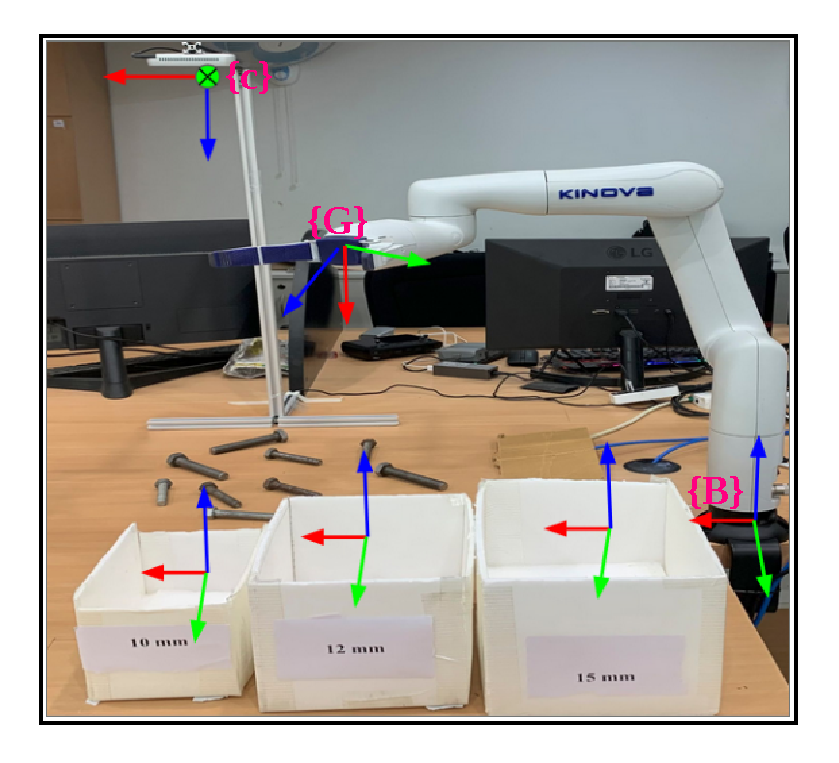
\includegraphics[width=0.6\textwidth]{Images/boltHandling/coordinate_frames.pdf}
\caption{Coordinate frames used throughout this chapter: the manipulator base frame $B$, the
gripper frame $G$, the globally mounted camera frame $C$.}
\label{fig:vp_frames}
\end{figure}

Both pipelines also convert between pixel coordinates and metric coordinates in the camera frame
using a shared pinhole model. Let $(u,v)$ denote pixel coordinates with origin at the top-left of
the image, $u$ increasing rightward and $v$ increasing downward, let $(u_0, v_0)$ denote the
principal point, and let $f_u$ and $f_v$ denote the focal length expressed in pixels along $u$ and
$v$ respectively, obtained from the sensor resolution $\mathrm{res}$ and field of view
$\mathrm{fov}$ by
\begin{equation}
f_u = \frac{\mathrm{res}_u}{2\tan(\mathrm{fov}_u/2)}, \qquad
f_v = \frac{\mathrm{res}_v}{2\tan(\mathrm{fov}_v/2)}.
\label{eq:vp_focal}
\end{equation}
Given the depth $Z$ at pixel $(u,v)$, the corresponding point in the camera frame is
\begin{equation}
X = \frac{u - u_0}{f_u}\,Z, \qquad Y = \frac{v - v_0}{f_v}\,Z, \qquad Z = Z,
\label{eq:vp_backproject}
\end{equation}
and, conversely, a length of $\mathrm{size}_{px}$ pixels measured at depth $Z$ corresponds to a
metric length
\begin{equation}
\mathrm{size}_{m} = \frac{\mathrm{size}_{px}}{f_u}\,Z.
\label{eq:vp_pixel2metric}
\end{equation}
Equation~\eqref{eq:vp_pixel2metric} is the relation used for size estimation in both
Section~\ref{sec:vp_template} and Section~\ref{sec:vp_segmentation}; what differs between the two
pipelines is how $\mathrm{size}_{px}$ itself is measured from the segmented image.

%% ============================================================
\section{Pipeline I: RGB-D Point-Cloud Segmentation with Oriented Chamfer Matching}\label{sec:vp_template}
%% ============================================================

The first pipeline targets the hardest instance of the sorting problem: bolts of unknown pose,
overlapping and touching one another inside a bin, with no prior instance segmentation available.
It was validated in an industrial shop-floor scene built in Gazebo (ROS1) with a globally
positioned RGB-D camera and a simulated Kinova Gen3 Lite arm, shown in
Figure~\ref{fig:vp_setup}~\citep{sk2024bolthandling}. Because template matching against a CAD
model is more tractable than learning a detector for objects with almost no discriminative
texture, and because a single reference template suffices for every bolt size, this pipeline
avoids both a training dataset and per-size template libraries.

\begin{figure}[htbp]
\centering
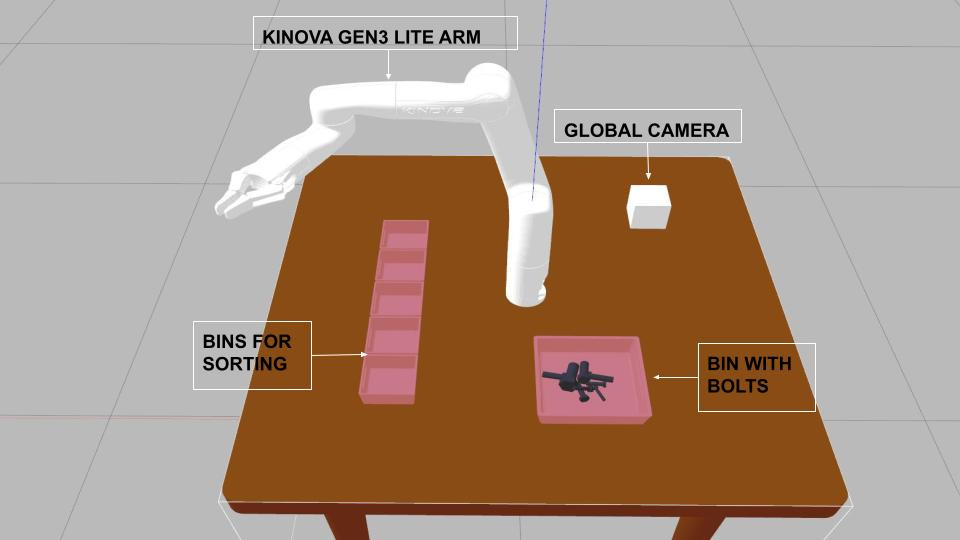
\includegraphics[width=\linewidth]{Images/boltHandling/gazebo_setup.jpg}
\caption{Experimental setup in the Gazebo shop-floor environment: a Kinova Gen3 Lite arm, a bin of
overlapping bolts of varying sizes, and a globally positioned RGB-D
camera~\citep{sk2024bolthandling}.}
\label{fig:vp_setup}
\end{figure}

The pipeline decomposes the sorting task into six phases: (1) RGB-D data acquisition, (2)
segmentation of the RGB image by $k$-means clustering, (3) data conditioning, (4) template matching
by Chamfer-distance minimization, (5) robotic manipulation, and (6) size estimation and sorting.
Phases 2--4 and 6 are detailed below; Phase 5 is standard MoveIt-based pick-and-place and is not
elaborated further.

%% ------------------------------------------------------------
\subsection{Search-Volume Restriction by \texorpdfstring{$k$}{k}-Means Segmentation}\label{subsec:vp_kmeans}
%% ------------------------------------------------------------

Conventional template matching searches the entire point cloud for a match, which is
computationally prohibitive for a scene containing dozens of overlapping bolts. Rather than search
blindly, the RGB frame is first segmented by $k$-means clustering with $k = 3$, corresponding to
the table, the bin, and the bolts, grouping pixels by intensity into these three clusters. The
resulting segmented image is thresholded into a binary mask, from which the individual bolt
contours are extracted (Figure~\ref{fig:vp_kmeans}). Point-cloud data corresponding to each
contour's minimum-area bounding rectangle is then extracted and downsampled with a voxel-grid
filter, restricting Phase 4 to a small search volume per candidate rather than the full scene
(Figure~\ref{fig:vp_searchvol}).

\begin{figure}[htbp]
\centering
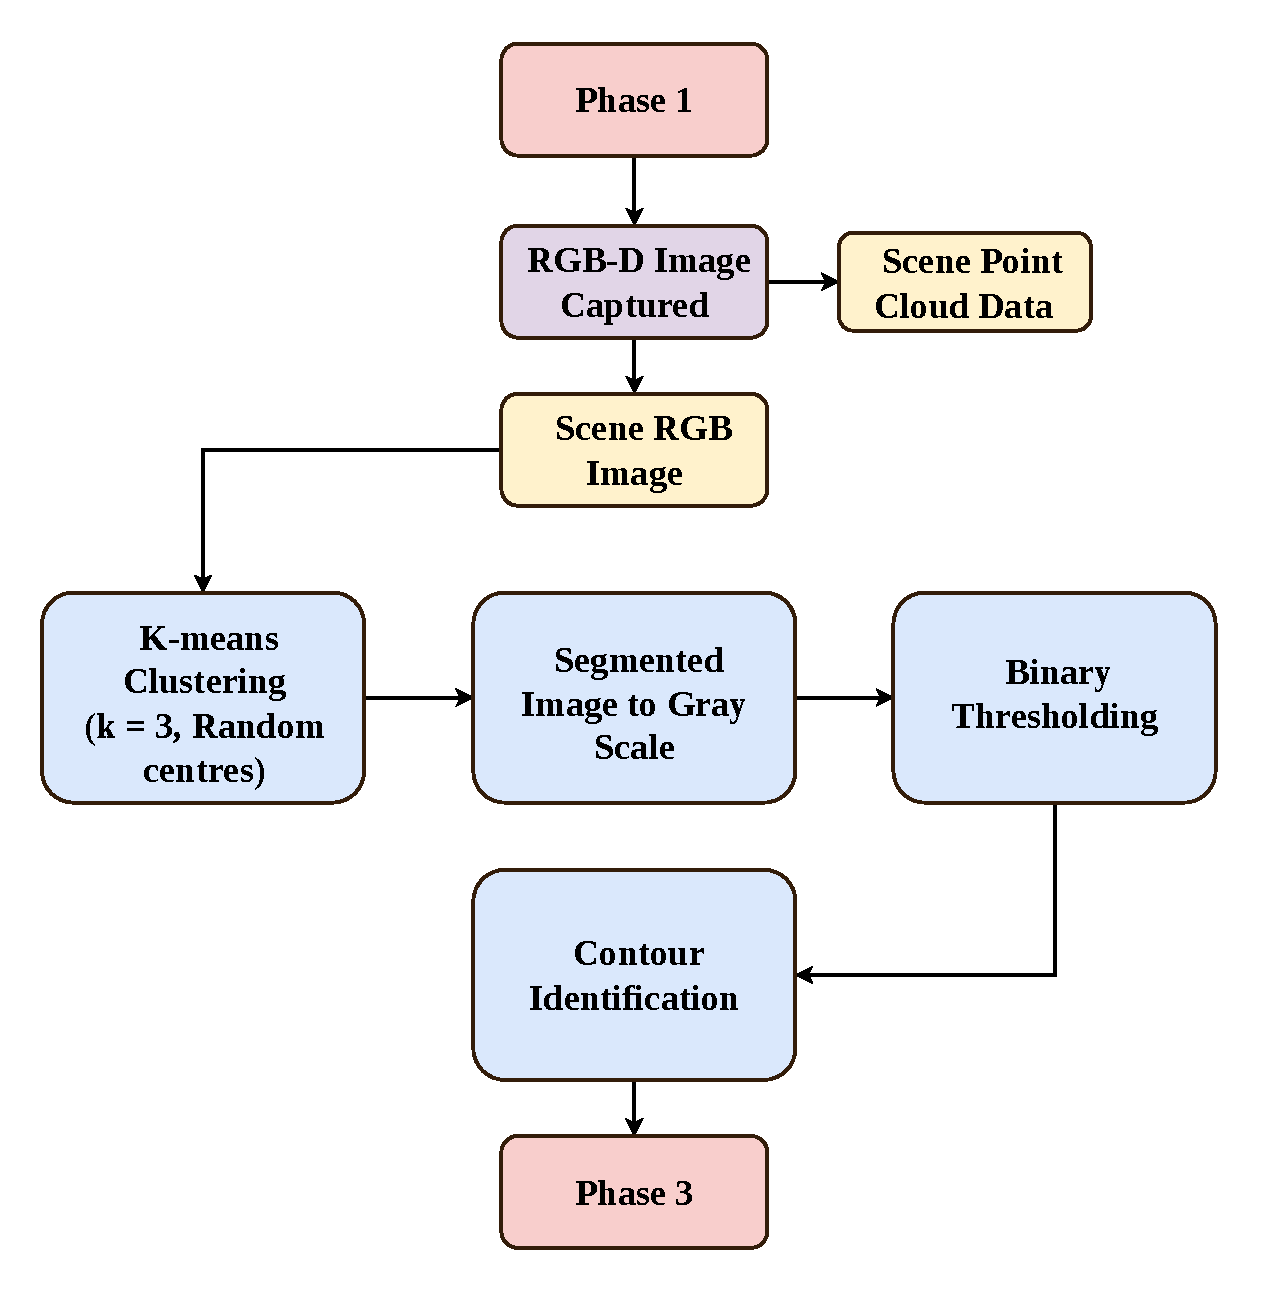
\includegraphics[width=0.75\linewidth]{Images/boltHandling/phase2_segmentation.pdf}
\caption{Segmentation of the captured RGB image by $k$-means clustering, isolating bolt contours
from the table and bin~\citep{sk2024bolthandling}.}
\label{fig:vp_kmeans}
\end{figure}

\begin{figure}[htbp]
\centering
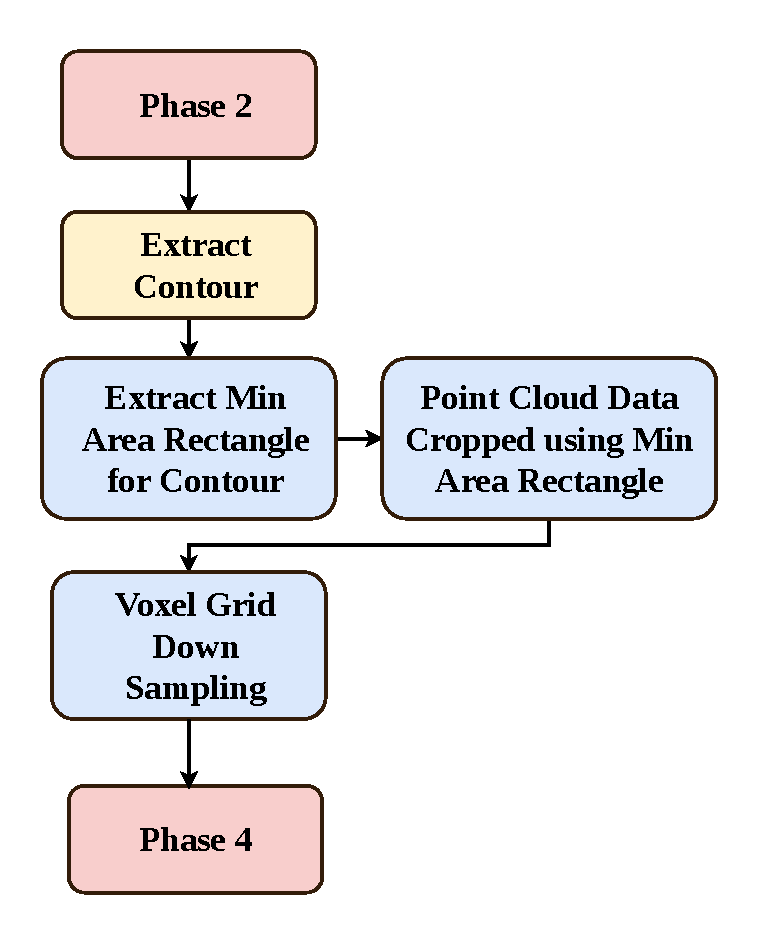
\includegraphics[width=0.5\linewidth]{Images/boltHandling/phase3_search_volume.pdf}
\caption{Extraction of the search volume from the captured scene: a minimum-area bounding rectangle around each contour restricts the point-cloud region passed to template matching~\citep{sk2024bolthandling}.}
\label{fig:vp_searchvol}
\end{figure}

%% ------------------------------------------------------------
\subsection{Oriented Chamfer Matching for Pose Estimation}\label{subsec:vp_chamfer}
%% ------------------------------------------------------------

For each restricted search volume, a reference bolt template with $N$ points is registered against
the scene point cloud. The template's centroid is first translated to a candidate scene point
$P_{j,s}$, and then incrementally rotated over the full range of yaw $\theta$ and pitch $\delta$
angles, $\theta, \delta \in [0^\circ, 360^\circ)$. Both angles are required, rather than a single
in-plane rotation, because bolts inside the bin can present at an arbitrary 3D tilt rather than
lying flat. For every candidate translation $j$ and angle pair $(\theta, \delta)$, the Chamfer
distance between the rotated template and the scene is computed as the sum of squared distances
from each template point $p_{i,t}$ to its nearest neighbour $c$ in the scene point cloud:
\begin{equation}
D(p_{j,s}, \theta, \delta) = \sum_{i=0}^{N} \left| \left( p_{i,t} - c \right)^2 \right|.
\label{eq:vp_chamfer}
\end{equation}
The pose estimate is the translation and orientation minimizing this distance over all candidate
positions in the search volume:
\begin{equation}
D^*(P_{j,s}, \theta, \delta) = \min_{j,\,\theta,\,\delta}\; D(p_{j,s}, \theta, \delta),
\label{eq:vp_chamfer_min}
\end{equation}
giving the feature vector
\begin{equation}
V = \left( P^C_o,\; \theta,\; \delta \right),
\label{eq:vp_featurevec}
\end{equation}
where $P^C_o$ is the position and $(\theta, \delta)$ the orientation of the matched bolt in the
camera frame, illustrated in Figure~\ref{fig:vp_matching} and Figure~\ref{fig:vp_pose}. The pose
$V$ is then carried into Equation~\eqref{eq:vp_transform} with $R^C_o = R^C_o(\theta, \delta)$ to
obtain the bolt's pose in the base frame for grasp planning
(Figure~\ref{fig:vp_manipulation}).

\begin{figure}[htbp]
\centering
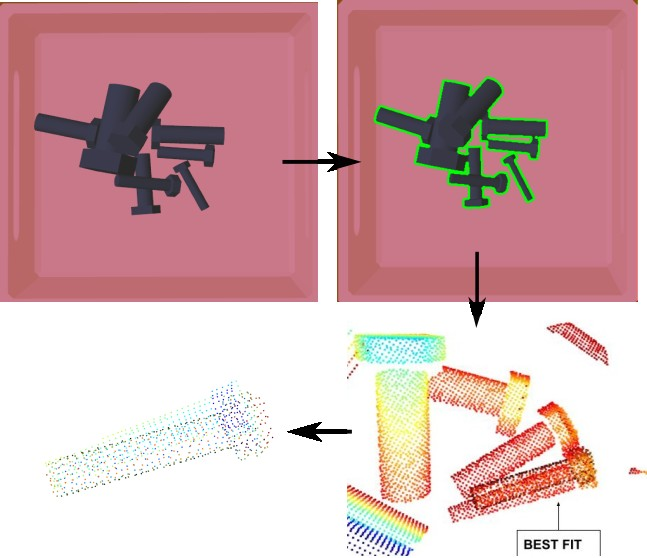
\includegraphics[width=0.65\linewidth]{Images/boltHandling/template_matching.jpeg}
\caption{Template match found on overlapping, densely configured bolts in the
bin~\citep{sk2024bolthandling}.}
\label{fig:vp_matching}
\end{figure}

\begin{figure}[htbp]
\centering
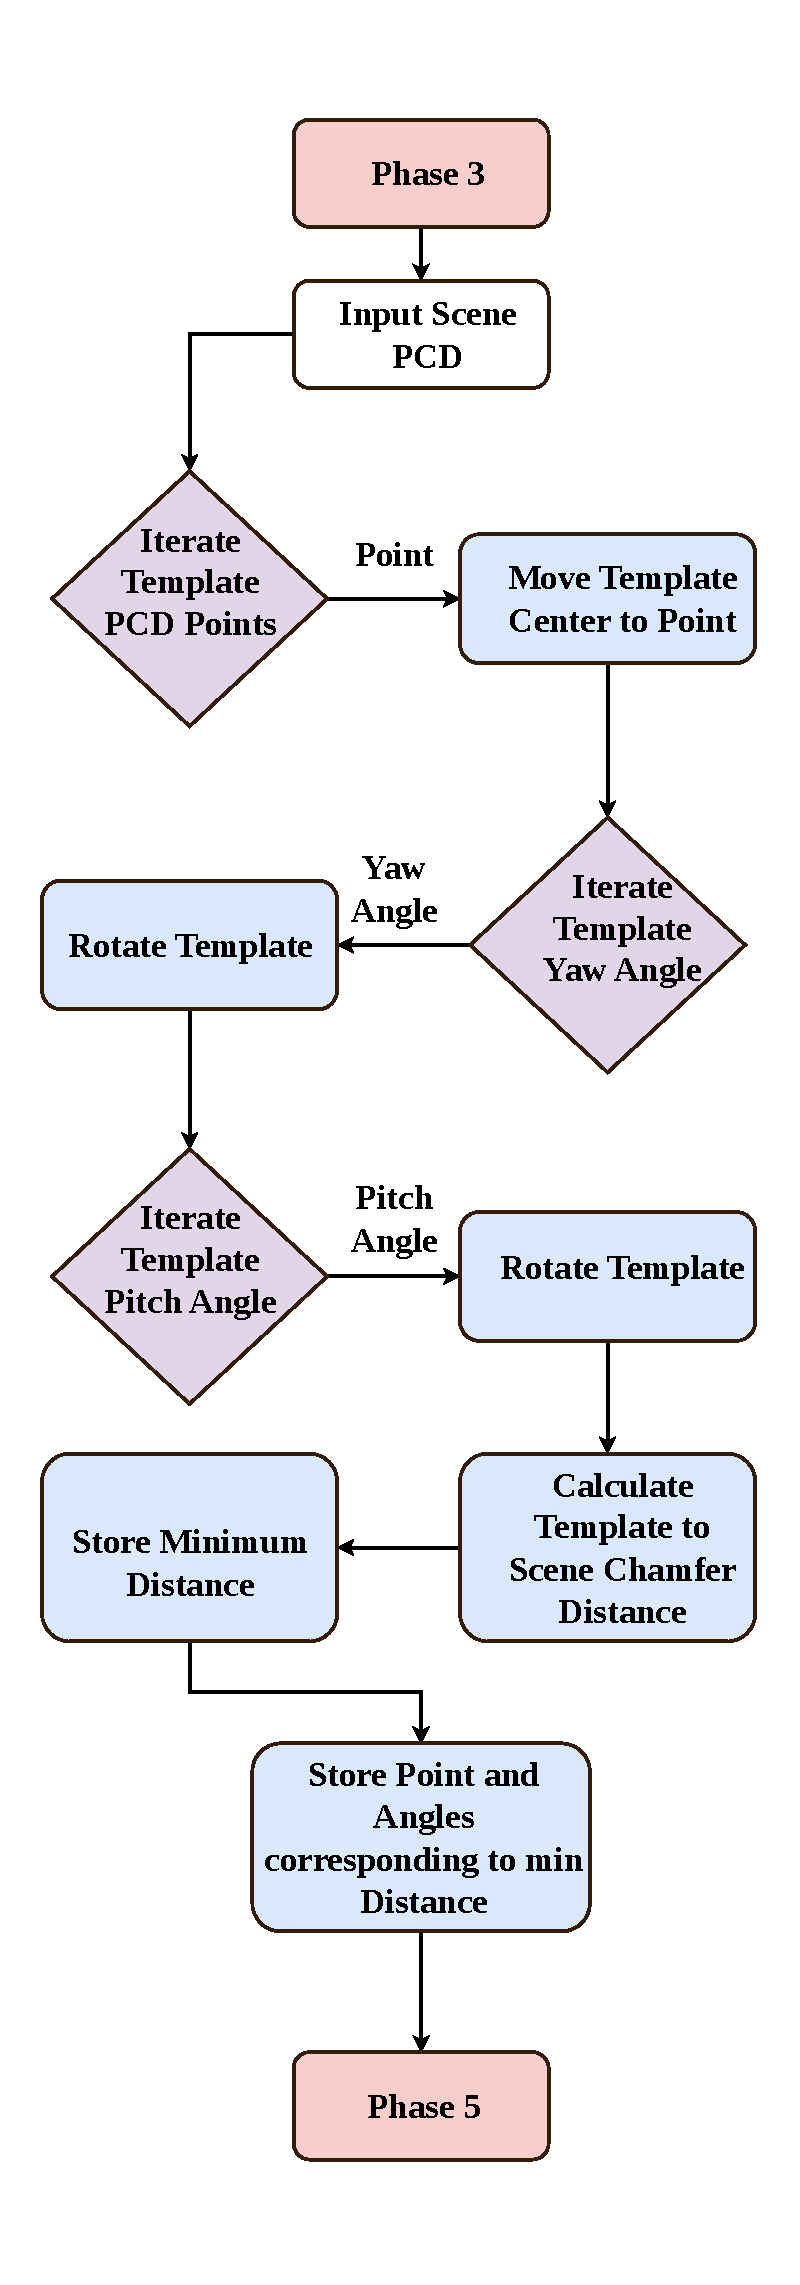
\includegraphics[width=0.5\linewidth]{Images/boltHandling/phase4_pose_estimation.pdf}
\caption{Rotational pose $(\theta, \delta)$ estimation of the bolt within the
bin~\citep{sk2024bolthandling}.}
\label{fig:vp_pose}
\end{figure}

\begin{figure}[htbp]
\centering
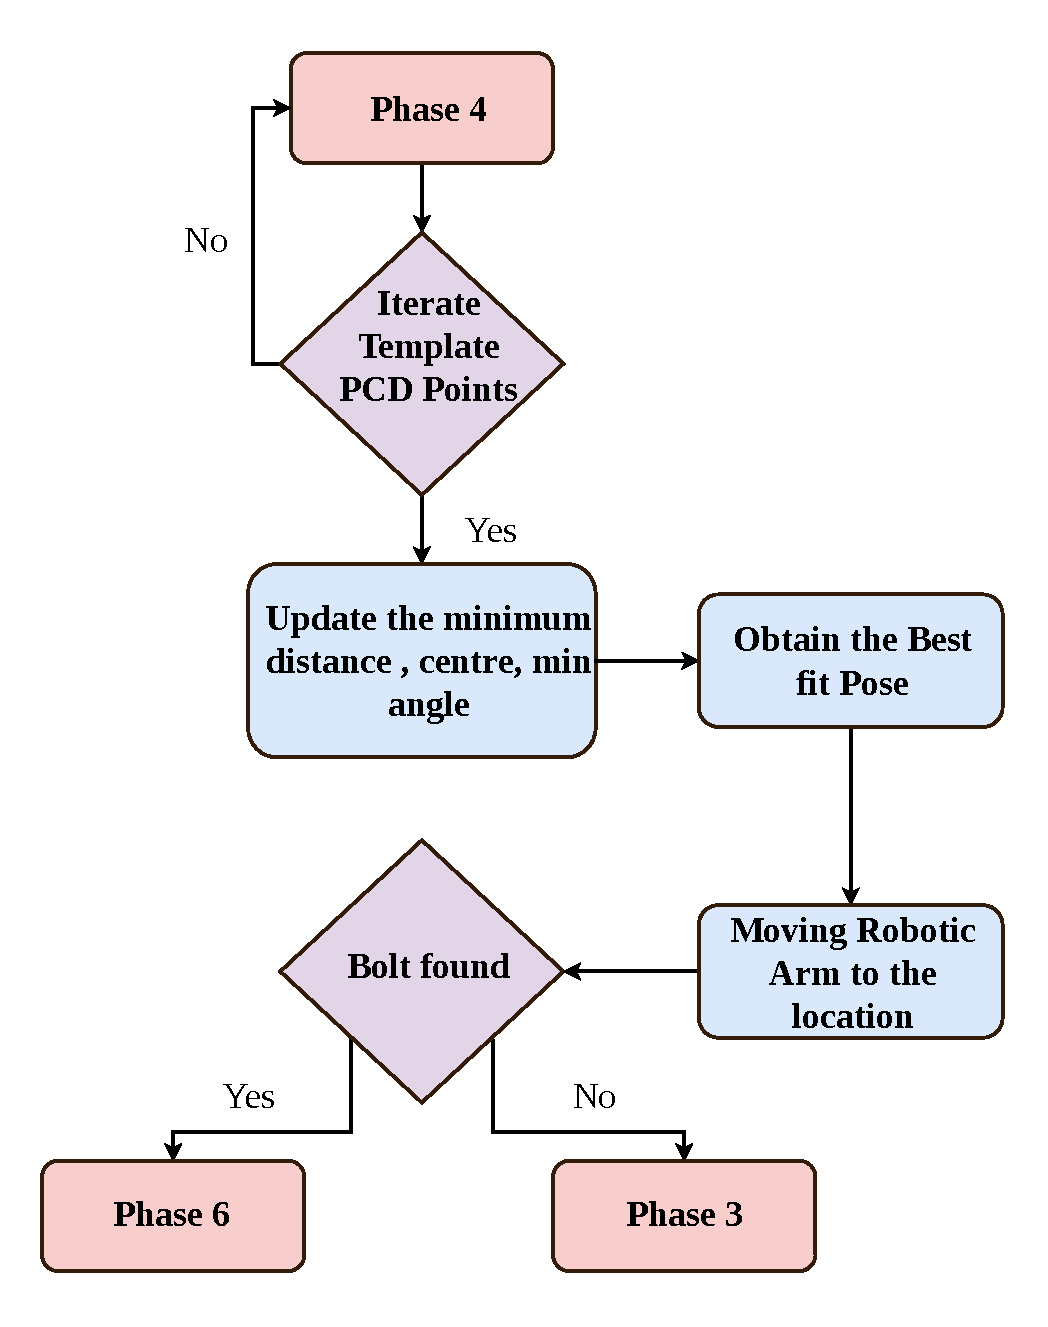
\includegraphics[width=0.5\linewidth]{Images/boltHandling/phase5_manipulation.pdf}
\caption{Robotic arm approaching the bin to pick up the bolt located by template
matching~\citep{sk2024bolthandling}.}
\label{fig:vp_manipulation}
\end{figure}

Pick-and-place with the resulting pose was validated under varying lighting conditions
(Figure~\ref{fig:vp_lighting}), since the search-volume restriction of
Section~\ref{subsec:vp_kmeans} depends on colour segmentation and is therefore the step most
exposed to illumination change.

\begin{figure}[htbp]
\centering
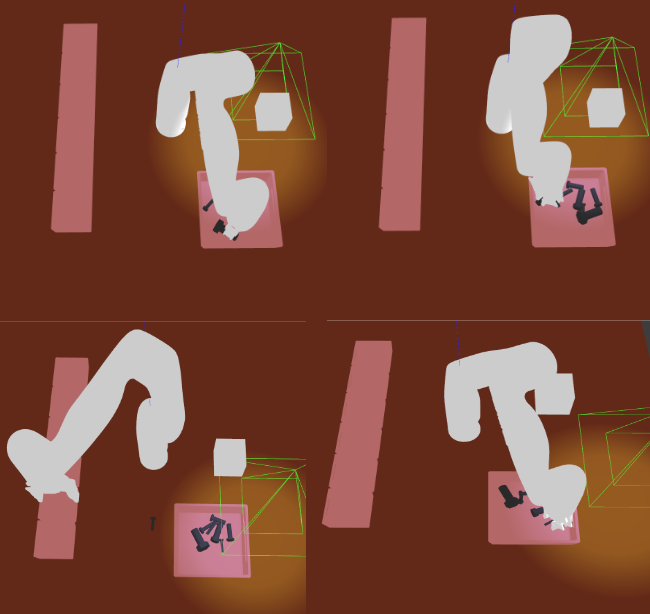
\includegraphics[width=0.65\linewidth]{Images/boltHandling/diff_lighting.png}
\caption{Pick-and-place of a bolt performed under varying lighting
conditions~\citep{sk2024bolthandling}.}
\label{fig:vp_lighting}
\end{figure}

%% ------------------------------------------------------------
\subsection{Colour-Based Size Estimation and Sorting}\label{subsec:vp_sizing1}
%% ------------------------------------------------------------

Once picked, the bolt is placed under the global camera for size estimation. Let $(c_u, c_v)$
denote the centroid of the bolt's contour in the binary segmented image, and let $(N_{Pu}, N_{Pv})$
denote the nearest point on the contour to that centroid, under the assumption that this nearest
point lies along the perpendicular from the centroid to the bolt head's edge
(Figure~\ref{fig:vp_sizing}). The bolt head radius in pixels is
\begin{equation}
R = \sqrt{\left(N_{Pu} - c_u\right)^2 + \left(N_{Pv} - c_v\right)^2},
\label{eq:vp_radius}
\end{equation}
giving a pixel diameter $\mathrm{size}_{px} = 2R$, which is converted to a metric diameter by
Equation~\eqref{eq:vp_pixel2metric} using the camera's known depth $Z$ to the placement surface and
the focal length $f_u$ from Equation~\eqref{eq:vp_focal}. The bolt is then routed to the bin
matching its estimated size, repeating for every bolt in the heap
(Figure~\ref{fig:vp_sizingalg}).

\begin{figure}[htbp]
\centering
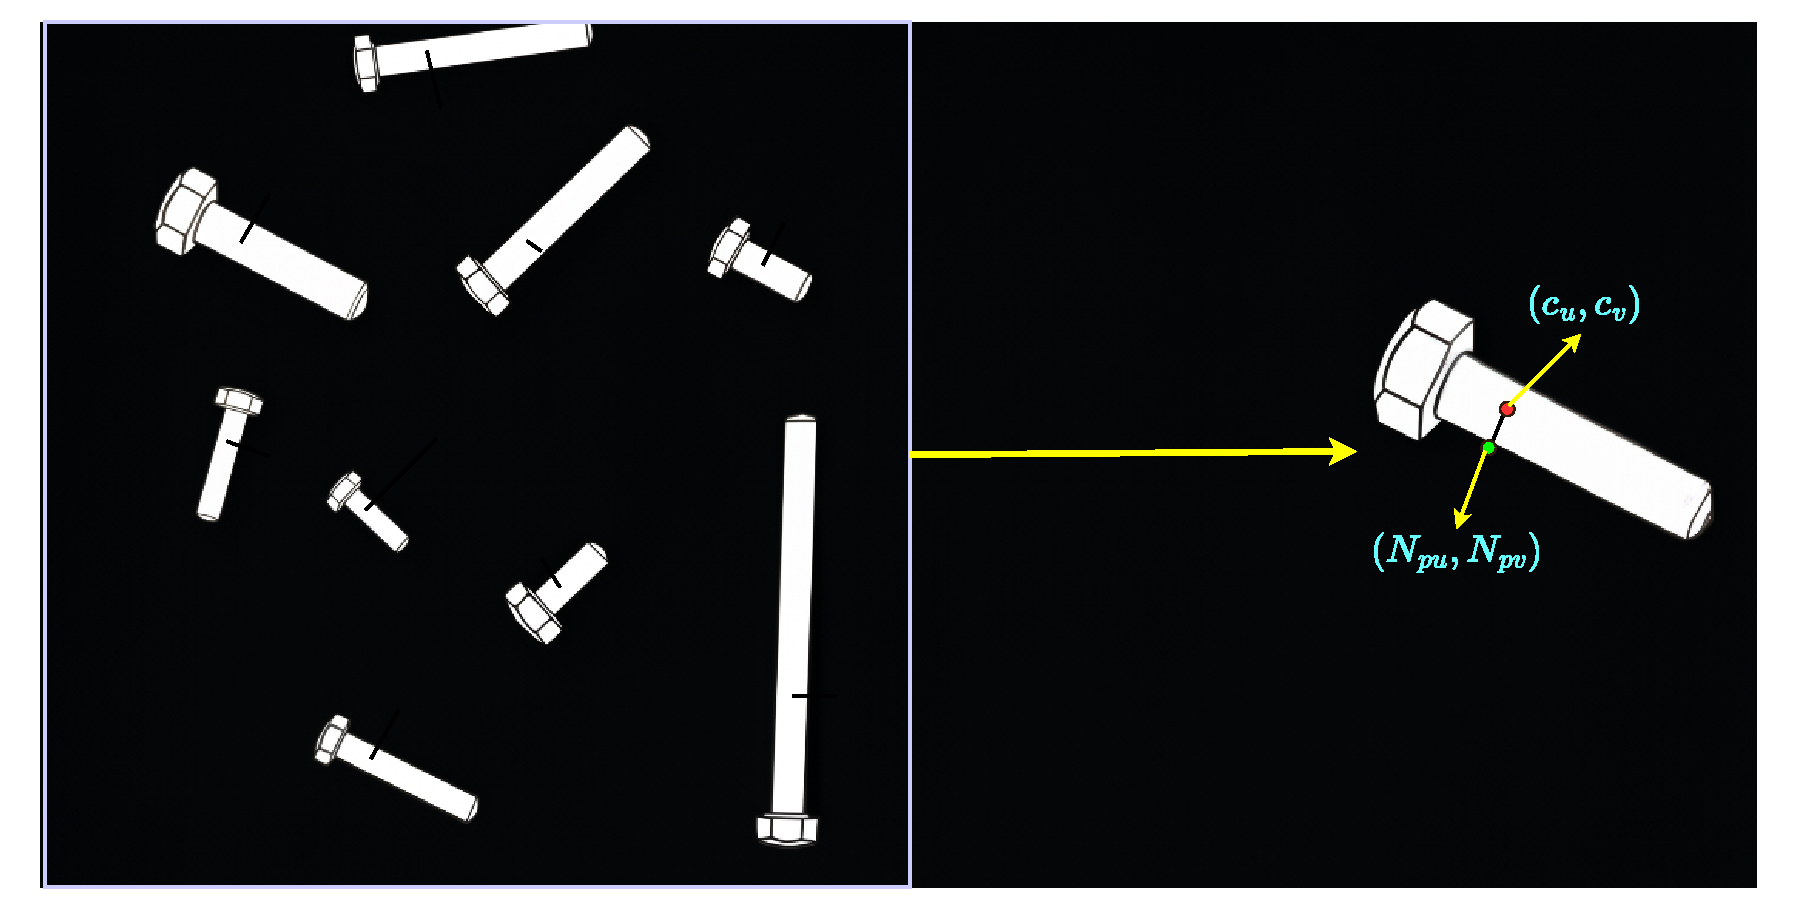
\includegraphics[width=0.9\linewidth]{Images/boltHandling/binary_image_size_estimation.pdf}
\caption{Size estimation of bolts detected from the bin: the radius $R$ is measured from the
contour centroid $(c_u, c_v)$ to the nearest contour point~\citep{sk2024bolthandling}.}
\label{fig:vp_sizing}
\end{figure}

\begin{figure}[htbp]
\centering
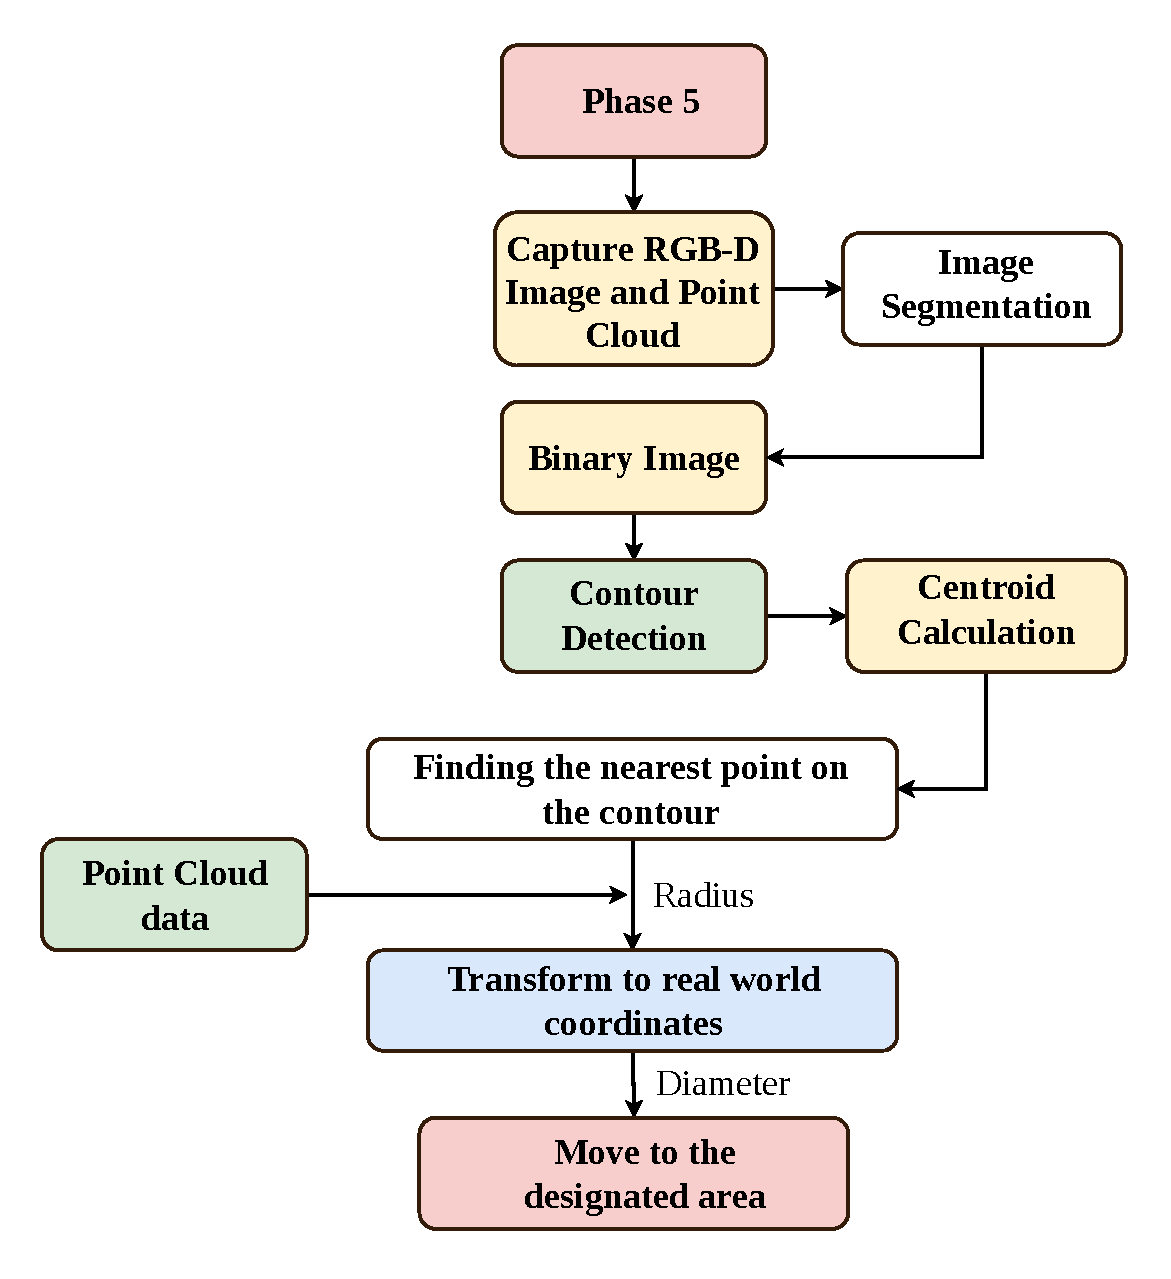
\includegraphics[width=0.55\linewidth]{Images/boltHandling/phase6_size_estimation.pdf}
\caption{Bolt size estimation algorithm, from contour extraction to sorting
decision~\citep{sk2024bolthandling}.}
\label{fig:vp_sizingalg}
\end{figure}

%% ------------------------------------------------------------
\subsection{Results}\label{subsec:vp_results1}
%% ------------------------------------------------------------

Table~\ref{tab:vp_poseerror} summarizes the localization accuracy achieved across a representative
sample of bolts spanning M6 to M20, with an RMS position error of 0.005\,m over the full
experiment. The error is attributed principally to the point-cloud downsampling step size used
during Chamfer matching and, to a lesser degree, to the fixed scale of the reference
template~\citep{sk2024bolthandling}.

\begin{table}[htbp]
\centering
\caption{Representative position estimation error, Pipeline I.}
\label{tab:vp_poseerror}
\begin{tabular}{lccc}
\toprule
\textbf{Bolt} & \textbf{Actual position (m)} & \textbf{Estimated position (m)} & \textbf{Error (m)} \\
\midrule
M6  & $[-0.110,\ 0.250,\ 0.553]$ & $[-0.109,\ 0.249,\ 0.557]$ & 0.004 \\
M8  & $[-0.122,\ 0.246,\ 0.556]$ & $[-0.121,\ 0.249,\ 0.558]$ & 0.003 \\
M10 & $[-0.103,\ 0.260,\ 0.559]$ & $[-0.100,\ 0.256,\ 0.556]$ & 0.005 \\
M12 & $[-0.055,\ 0.245,\ 0.558]$ & $[-0.058,\ 0.243,\ 0.563]$ & 0.006 \\
M16 & $[-0.088,\ 0.212,\ 0.559]$ & $[-0.085,\ 0.211,\ 0.563]$ & 0.005 \\
M20 & $[-0.070,\ 0.238,\ 0.563]$ & $[-0.068,\ 0.237,\ 0.565]$ & 0.003 \\
\bottomrule
\end{tabular}
\end{table}

Size estimation reached an accuracy of 0.36\,mm RMS error, sufficient to distinguish adjacent
metric bolt sizes. The dominant error source is the discrete nature of pixel sampling when locating
the nearest contour point in Equation~\eqref{eq:vp_radius}: this discretization error is amplified
when converted to metric units by Equation~\eqref{eq:vp_pixel2metric}, and diminishes as camera
resolution increases~\citep{sk2024bolthandling}. Across all trials, the pipeline achieved bolt
sorting from a heap of overlapping bolts without any misclassification.

%% ============================================================
\section{Pipeline II: Deep-Learning Segmentation with Depth Fusion}\label{sec:vp_segmentation}
%% ============================================================

The second pipeline targets a complementary regime: bolts presented individually or loosely
scattered rather than densely overlapping, where a learned segmentation network can substitute for
the $k$-means and Chamfer stages of Section~\ref{sec:vp_template} to improve robustness to
background colour, lighting, and bolt ageing. It was validated on hardware with a Kinova Gen3 Lite
arm and an Intel RealSense D415 RGB-D camera~\citep{sk2024boltsorting}. The pipeline integrates
four components: object segmentation by a DeepLabV3+, size estimation by classical vision applied to the
segmented mask, localization in the robot's configuration, and robot reaching, summarized in
Figure~\ref{fig:vp_overview}.

\begin{figure}[htbp]
\centering
% \FigPlaceholder{0.75\linewidth}{Overall pipeline: RGB frame $\rightarrow$ semantic segmentation
% $\rightarrow$ image-frame localization $(u, v, \theta)$ $\rightarrow$ camera-frame transform
% $(X, Y, Z, \theta)$ $\rightarrow$ base-frame transform $(X', Y', Z', \theta')$ $\rightarrow$
% Kinova API $\rightarrow$ sorting; aligned depth feeds size estimation in parallel with
% localization. Source figure archived only in the published manuscript; reproduce from Fig.~1 of
% \citet{sk2024boltsorting}.}
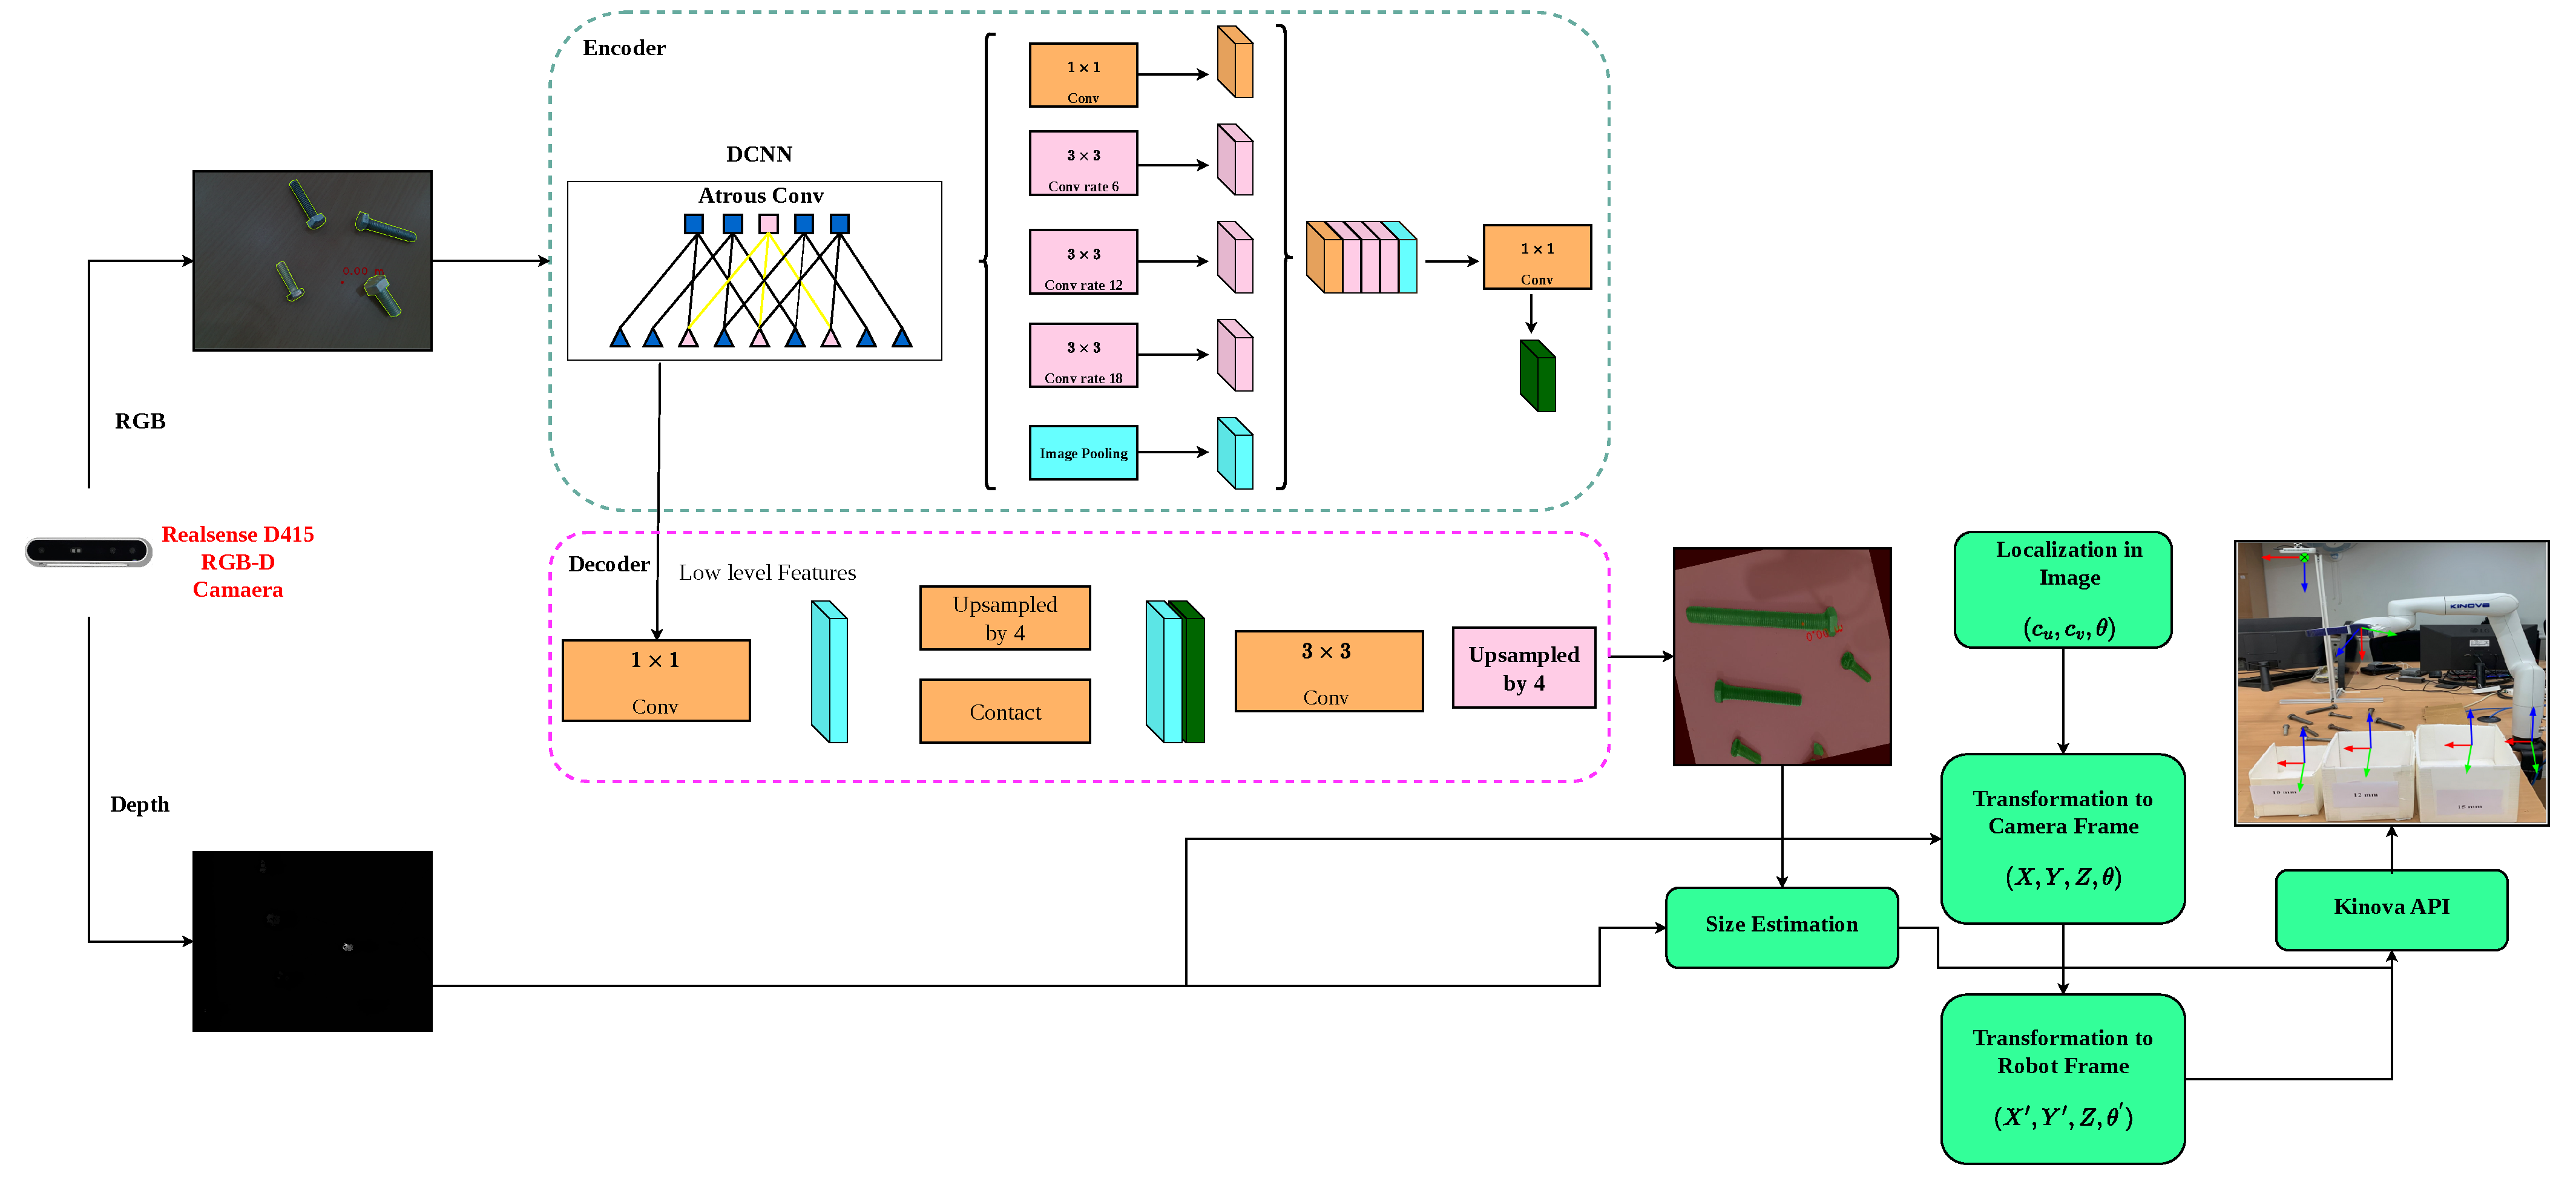
\includegraphics[width=\linewidth]{Images/case/overall_methodology.pdf}
\caption{Overall methodology of Pipeline II, from RGB-D acquisition to sorted
placement~\citep{sk2024boltsorting}.}
\label{fig:vp_overview}
\end{figure}

%% ------------------------------------------------------------
\subsection{Custom Dataset and Semantic Segmentation}\label{subsec:vp_dataset}
%% ------------------------------------------------------------

Unlike Section~\ref{sec:vp_template}, which requires no training data, this pipeline is
learning-based and therefore begins with a custom bolt dataset. Images ($480 \times 640$) were
collected under varying backgrounds (green, blue, black, cemented tile, and wooden-table surfaces)
and varying illumination (daylight and laboratory lighting), including both new and aged
mild-steel bolts, to cover the environmental variation that degrades the colour-based segmentation
of Section~\ref{subsec:vp_kmeans}. The resulting 2000-image dataset, including augmentations, was
annotated and split 80/10/10 into training, test, and validation sets~\citep{sk2024boltsorting}.

% \begin{figure}[htbp]
% \centering
% \FigPlaceholder{0.75\linewidth}{(a) Sample data-collection frames across background and lighting
% conditions. (b) Corresponding polygon annotations of bolts. Source figure archived only in the
% published manuscript; reproduce from Fig.~2 of \citet{sk2024boltsorting}.}
% \caption{Data collection and annotation for the custom bolt dataset~\citep{sk2024boltsorting}.}
% \label{fig:vp_dataset}
% \end{figure}

\begin{figure}[htbp]
    \begin{subfigure}{0.4\textwidth}
        \centering
        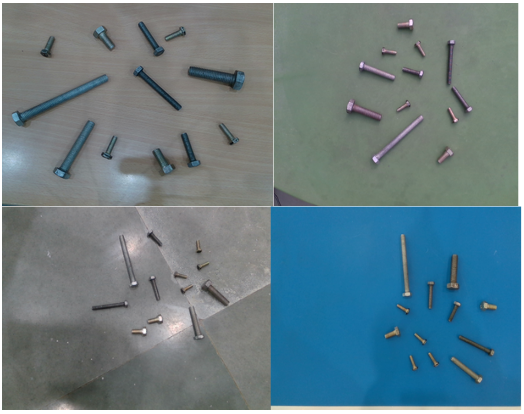
\includegraphics[width=1\linewidth]{Images/case/paper_1.png}
        \caption{}
        \label{fig:figure_a}
    \end{subfigure}
    \hfill
    \begin{subfigure}{0.425\textwidth}
        \centering
        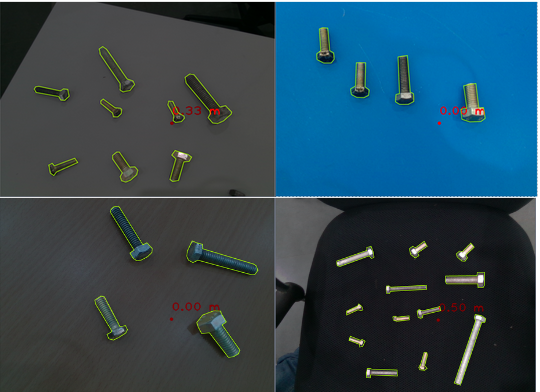
\includegraphics[width=1\linewidth]{Images/case/paper_2.png} 
        \caption{}
        \label{fig:figure_b}
    \end{subfigure}
    \caption{(a) Data collection (b) Annotations of custom bolt dataset~\citep{sk2024boltsorting}.}
    \label{fig:combined_figures}
\end{figure}

Four semantic segmentation architectures were evaluated on this dataset: PPLiteSeg with its STDC~I
and STDC~II backbones, OCRNet with an HRNet-48w backbone, and DeepLabV3+ with a ResNet101
backbone. Because the objective is to sort by size rather than to distinguish individual bolt
instances, semantic segmentation, which assigns a single label to all bolts in the frame, is
sufficient and computationally cheaper than instance
segmentation~\citep{sk2024boltsorting}. Table~\ref{tab:vp_segcompare} reports the comparison.
DeepLabV3+'s atrous spatial pyramid pooling aggregates context at multiple scales, which is
particularly effective for the diverse sizes and orientations bolts present in the dataset, and its
ResNet101 backbone yields the highest mIoU, Dice coefficient, and Cohen's Kappa score of the four
architectures, at the cost of a larger model than the two PPLiteSeg variants.

\begin{table}[htbp]
\centering
\caption{Comparison of segmentation architectures on the custom bolt dataset.}
\label{tab:vp_segcompare}
\resizebox{\textwidth}{!}{%
\begin{tabular}{lcccc}
\toprule
\textbf{Model} & \textbf{PPLiteSeg~I}~\citep{peng2022pp} & \textbf{PPLiteSeg~II}~\citep{peng2022pp} & \textbf{DeepLabV3+}~\citep{chen2018encoder} & \textbf{OCRNet}~\citep{yuan2020object} \\
\midrule
Backbone            & STDC~I & STDC~II & ResNet101\_vd & HRNet-48w \\
mIoU                & 0.8921 & 0.8964  & \textbf{0.92}  & 0.9135 \\
Model size (MB)     & 31.8   & 47.2    & 174            & 268 \\
Inference time (ms) & 228    & 330     & \textbf{131}   & 275 \\
Dice coefficient    & 0.9399 & 0.9427  & \textbf{0.9568}& 0.9530 \\
Kappa score         & 0.8797 & 0.8855  & \textbf{0.9136}& 0.9060 \\
\bottomrule
\end{tabular}%
}
\end{table}

\begin{figure}[htbp]
\centering
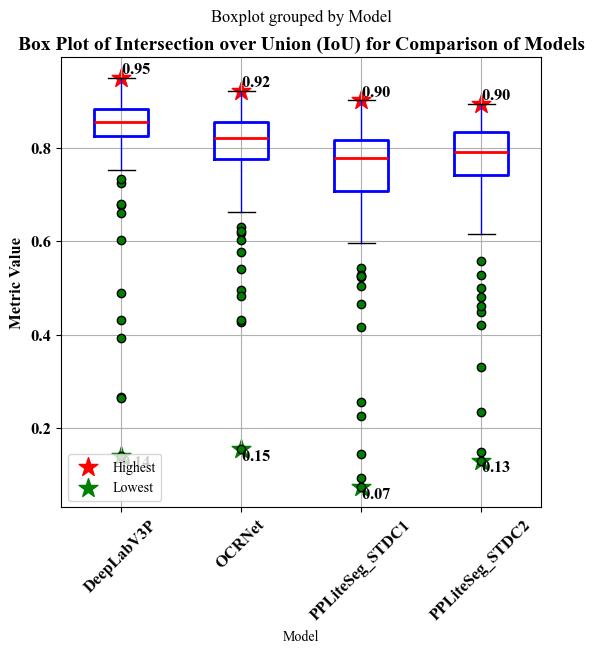
\includegraphics[width=0.85\linewidth]{Images/case/iou_comparison.png}
% \FigPlaceholder{0.6\linewidth}{Boxplot of per-image IoU by model, annotating the highest (0.95) and
% lowest per-sample scores for each architecture. Source figure archived only in the published
% manuscript; reproduce from Fig.~3 of \citet{sk2024boltsorting}.}
\caption{Distribution of per-image IoU scores across the evaluated
architectures~\citep{sk2024boltsorting}.}
\label{fig:vp_ioubox}
\end{figure}

The comparatively low outlier scores visible in the per-image IoU distribution
(Figure~\ref{fig:vp_ioubox}) are attributable to backgrounds with colour close to the bolts,
extended shadows obscuring bolt boundaries, and augmented images containing variation not present
in training~\citep{sk2024boltsorting}.

%% ------------------------------------------------------------
\subsection{Depth-Fused Localization and Size Estimation}\label{subsec:vp_sizing2}
%% ------------------------------------------------------------

Once the RGB frame is segmented, the aligned depth frame provides the metric information needed
for both localization and sizing. Let $(c_u, c_v)$ denote the centroid of a segmented bolt in the
image, and let $D_{px}$ denote the width, in pixels, of the minimum-area bounding box fitted to the
bolt's mask, corresponding to the bolt head diameter. The bolt's
in-plane orientation $\theta$ is taken as the inclination of the bounding box's longest side to the
horizontal $u$-axis. Unlike the two-angle pose of Equation~\eqref{eq:vp_featurevec}, a single angle
suffices here because the bolt lies flat under the global camera rather than at an arbitrary tilt
inside a bin.

% \begin{figure}[htbp]
% \centering
% 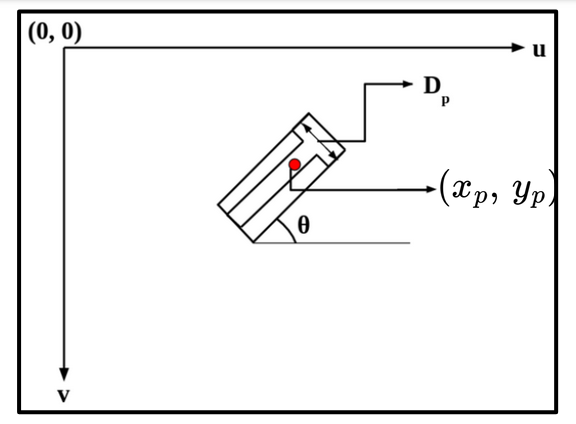
\includegraphics[width=\linewidth]{Images/case/segmented_bolt.png}
% % \FigPlaceholder{0.5\linewidth}{Pixel frame with origin at $(0,0)$, axes $u$ (right) and $v$ (down);
% % bounding-box diameter $D_{px}$, centroid $(c_u, c_v)$, and orientation $\theta$ of the segmented
% % bolt head. Source figure archived only in the published manuscript; reproduce from Fig.~5 of
% % \citet{sk2024boltsorting}.}
% \caption{Feature extraction from a segmented bolt image, Pipeline II.}
% \label{fig:vp_feature}
% \end{figure}

The bolt shank diameter in pixels is obtained by
\begin{equation}
d_{px} = \frac{D_{px}}{1.8},
\label{eq:vp_shankpx}
\end{equation}
the empirical head-to-shank ratio for the metric bolt geometry used in this dataset, and converted
to a metric shank diameter by the same pinhole relation as Section~\ref{subsec:vp_sizing1},
Equation~\eqref{eq:vp_pixel2metric}:
\begin{equation}
d_m = \frac{d_{px}}{f_u}\,Z.
\label{eq:vp_shankm}
\end{equation}
In parallel, the bolt's position in the camera frame is recovered from its pixel centroid and the
aligned depth using the shared back-projection of Equation~\eqref{eq:vp_backproject}, giving a
per-bolt feature vector analogous to Equation~\eqref{eq:vp_featurevec} but with a single orientation
angle,
\begin{equation}
V_i = \left( d_{m,i},\; X_i,\; Y_i,\; Z_i,\; \theta_i \right),
\label{eq:vp_featurevec2}
\end{equation}
for the $i^{\text{th}}$ segmented bolt (Figure~\ref{fig:vp_segoutput}).

\begin{figure}[htbp]
\centering
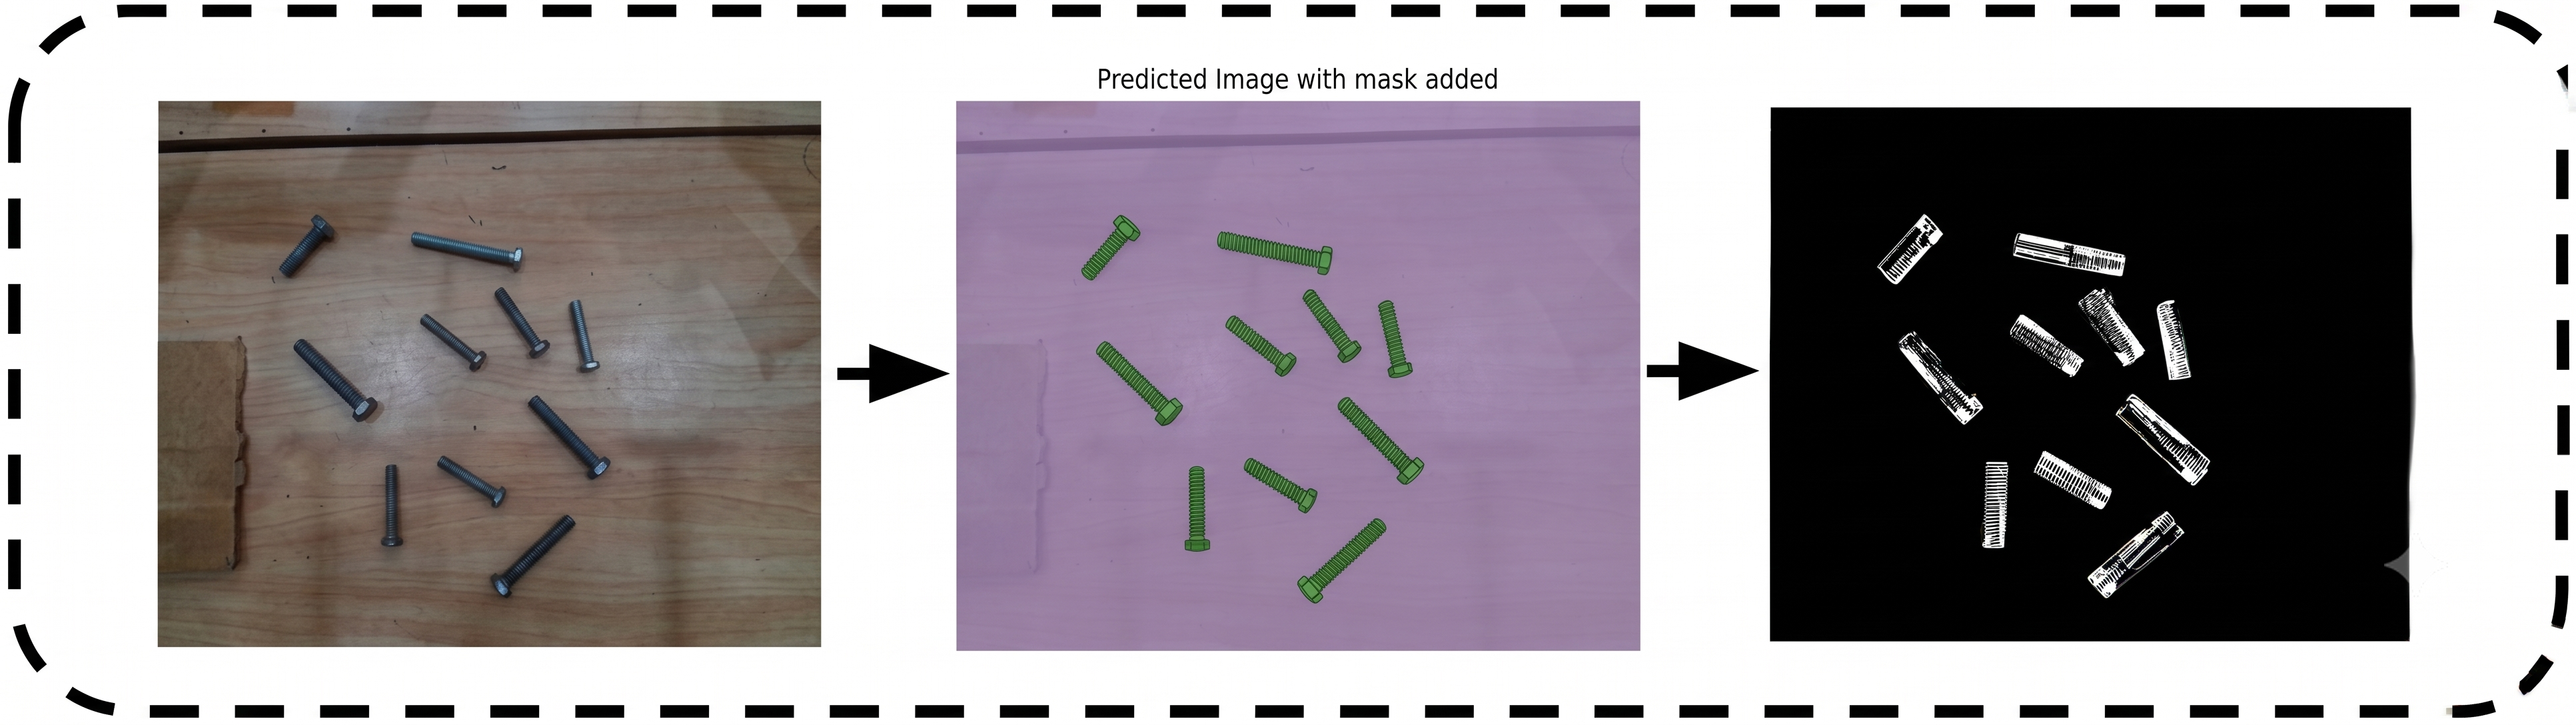
\includegraphics[width=0.75\linewidth]{Images/case/seg_output.png}
% \FigPlaceholder{}{RGB frame (left), semantic segmentation mask (middle), and binary
% mask with fitted bounding box and centreline (right) for the target bolts. Source figure archived
% only in the published manuscript; reproduce from Fig.~6 of \citet{sk2024boltsorting}.}
\caption{Segmentation output at each stage, from RGB frame to bounding-box feature
extraction~\citep{sk2024boltsorting}.}
\label{fig:vp_segoutput}
\end{figure}

%% ------------------------------------------------------------
\subsection{Localization in the Robot's Configuration}\label{subsec:vp_localization2}
%% ------------------------------------------------------------

With the camera and robot base at predefined, calibrated positions, the bolt's position in the
camera frame, $P^C_o = [X, Y, Z, 1]^\top$, is mapped to the base frame by
Equation~\eqref{eq:vp_transform}, specialized to a purely translational calibration offset
consistent with the fixed camera mount used in this setup:
\begin{equation}
P^B_o = T^B_C \cdot P^C_o, \qquad P^B_o = \left[ X',\ Y',\ Z,\ 1 \right]^\top.
\label{eq:vp_pose_transform2}
\end{equation}
This localization step is applied independently to every detected bolt, so that for $n$ bolts
detected in a single frame the transform is applied column-wise,
\begin{equation}
\begin{bmatrix}
X'^B_1 & \cdots & X'^B_n \\
Y'^B_1 & \cdots & Y'^B_n \\
Z'^B_1 & \cdots & Z'^B_n \\
1      & \cdots & 1
\end{bmatrix}
= T^B_C \cdot
\begin{bmatrix}
X^C_1 & \cdots & X^C_n \\
Y^C_1 & \cdots & Y^C_n \\
Z^C_1 & \cdots & Z^C_n \\
1     & \cdots & 1
\end{bmatrix}.
\label{eq:vp_nbolts}
\end{equation}
The resulting base-frame pose and orientation $(X', Y', Z, \theta')$ for each bolt is sent to the
manipulator as a control target via the Kinova API~\citep{sk2024boltsorting}.

%% ------------------------------------------------------------
\subsection{Sorting Criterion and Results}\label{subsec:vp_results2}
%% ------------------------------------------------------------

Each bolt's estimated shank diameter $d_m$ is mapped to a size class by a heuristic threshold rule:
\begin{equation}
\mathrm{bolt} =
\begin{cases}
\mathrm{M15} & \text{if } 13.5 \leq d_m < 16.5 \\
\mathrm{M12} & \text{if } 10.5 \leq d_m < 12.5 \\
\mathrm{M10} & \text{if } 9.5 \leq d_m < 10.3 \\
\mathrm{M8}  & \text{if } 7.0 \leq d_m < 8.5
\end{cases}
\label{eq:vp_sortrule}
\end{equation}
and the manipulator places the bolt in the corresponding bin. Table~\ref{tab:vp_sizeerror}
summarizes the estimation error across sample bolts of each class.

\begin{table}[htbp]
\centering
\caption{Error analysis of bolt size estimation across varying spatial positions over five experimental trials. Pipeline II.}
\label{tab:vp_sizeerror}
\begin{tabular}{lccc}
\toprule
\textbf{Class} & \textbf{Actual (mm)} & \textbf{Predicted, range (mm)} & \textbf{Error, range (mm)} \\
\midrule
M15 & 15 & 14.707 $\pm$ 1.284 & 1.005 $\pm$ 0.645\\
M12 & 12 & 11.725 $\pm$ 0.635 & 0.441 $\pm$ 0.498\\
M10 & 10 & 10.147 $\pm$ 0.157 & 0.187 $\pm$ 0.083\\
M8  & 8  & 8.026 $\pm$ 0.672  & 0.493 $\pm$ 0.358\\
\bottomrule
\end{tabular}
\end{table}

Across all trials, the DeepLabV3+ segmentation and depth-fusion pipeline localized and sorted bolts
with an mean error range of $0.187$ to $1.005$\,mm and a segmentation inference time of 130\,ms per
frame, without misclassifications, including bolt sizes not present in the training
set~\citep{sk2024boltsorting}. Figure~\ref{fig:vp_sortingresult} shows the resulting sorting
operation.

\begin{figure}[htbp]
\centering
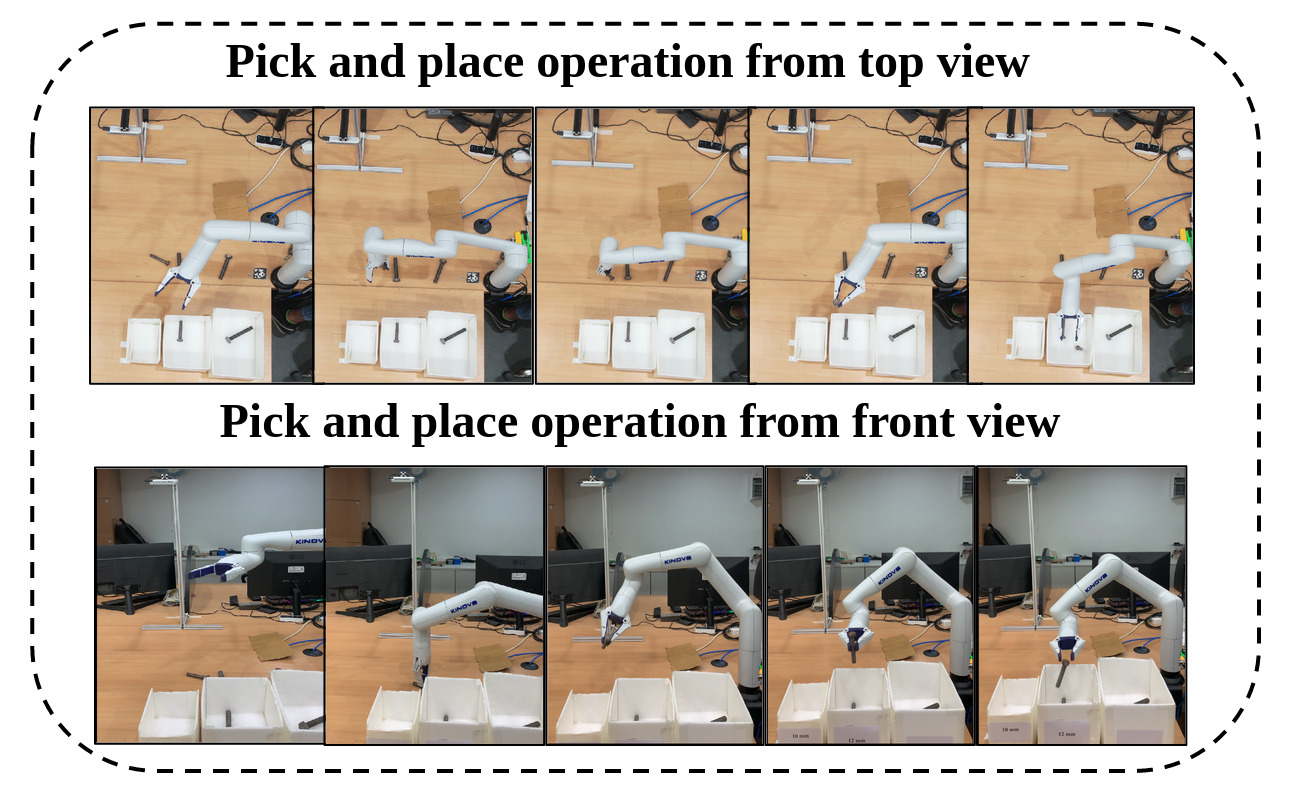
\includegraphics[width=\linewidth]{Images/case/end_results.jpg}
% \FigPlaceholder{0.75\linewidth}{Sequence of pick-and-place operations sorting bolts into their
% size-labelled bins, shown from the top and front views. Source figure archived only in the
% published manuscript; reproduce from Fig.~9 of \citet{sk2024boltsorting}.}
\caption{Picking and placing bolts into their respective size bins, Pipeline
II~\citep{sk2024boltsorting}.}
\label{fig:vp_sortingresult}
\end{figure}

%% ============================================================
\section{Comparison of the Two Pipelines}\label{sec:vp_comparison}
%% ============================================================

Both pipelines share the notation and pinhole projection of Section~\ref{sec:vp_notation}, the
same manipulator and calibrated camera-to-base transform $T^B_C$, and the same terminal output, a
pose and size estimate in the base frame consumed downstream by the manipulation stage. They differ
in the regime each targets, summarized in Table~\ref{tab:vp_pipelinecompare}.

\begin{table}[htbp]
\centering
\caption{Comparison of the two vision pipelines presented in this chapter.}
\label{tab:vp_pipelinecompare}
\resizebox{\textwidth}{!}{%
\begin{tabular}{lll}
\toprule
& \textbf{Pipeline I (Section~\ref{sec:vp_template})} & \textbf{Pipeline II (Section~\ref{sec:vp_segmentation})} \\
\midrule
Segmentation      & $k$-means clustering, no training data & DeepLabV3+~\citep{chen2018encoder}, custom-trained on 2000 images \\
Bolt configuration & Overlapping, arbitrary 3D tilt in a bin & Singulated, presented flat to the camera \\
Pose search        & Full $(\theta, \delta)$ Oriented Chamfer Matching & Bounding-box angle $\theta$ from the mask \\
Size cue           & Contour-to-centroid radius $R$ & Bolt head diameter $D_{px}$ \\
Sensitivity        & Colour segmentation, hence lighting-sensitive & Learned features, robust to bolt ageing \\
Validation platform & Gazebo (ROS1) simulation & Hardware, Kinova Gen3 Lite + RealSense D415 \\
Position/size error & 0.005\,m RMS / 0.36\,mm RMS & $-1.424$ to $1.655$\,mm \\
\bottomrule
\end{tabular}%
}
\end{table}

Pipeline I requires no training data and directly handles the overlapping, arbitrarily tilted
configurations that occur when bolts are dumped into a bin together, but its reliance on
colour-based $k$-means segmentation to restrict the Chamfer search volume ties its robustness to
lighting conditions. Pipeline II trades that training-free property for robustness to bolt ageing
and background variation, learned directly from a custom dataset, but assumes bolts are singulated
and presented flat, restricting its pose estimate to a single in-plane angle rather than the full
two-angle tilt Pipeline I recovers. In practice, the two are complementary stages of the same
sorting task: Pipeline I is suited to the initial, cluttered picking stage, and Pipeline II to a
subsequent, controlled sizing stage once a bolt has been singulated, which is the arrangement
validated on hardware in Section~\ref{subsec:vp_results2}.

The perception module developed in this chapter, in either configuration, returns a bolt pose in
the manipulator's base frame at the rate of a single eye-in-hand or globally mounted camera.
Chapter~\ref{chap:shared_vision} builds on exactly this output to address gap G2: when two arms share a workspace and
either arm's camera can observe a target, which arm should be assigned to reach it.
